\pdfminorversion=4
\documentclass[aspectratio=169,8pt]{beamer}
% Could add [8pt], 9, 10 11 12 14 17 20
% Font size can be \Huge \huge \LARGE \Large \large 
% \normalsize (default) \small \footnotesize \scriptsize\tiny
\usepackage[T1]{fontenc}
\usepackage[utf8]{inputenc}
\usepackage{lmodern}
\usepackage{hyperref}
\usetheme{Frankfurt}
\usepackage{listings}
\lstset{language=C,numbers=left,stepnumber=1,basicstyle=\ttfamily\scriptsize}
\usepackage[]{algorithm2e}
\newcommand*\lstinputpath[1]{\lstset{inputpath=#1}}
\newcommand{\R}[2]{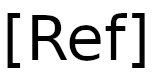
\includegraphics[height=.2cm]{IMG/Ref}\href{#2}{#1}}
\newcommand{\Y}[2]{
\includegraphics[height=.2cm]{IMG/YouTube}\href{https://www.youtube.com/watch?v=#2}{#1}}

% Other themes :default Darmstadt Malmoe AnnArbor Dresden Marburg Antibes
% Frankfurt Montpellier Bergen Goettingen PaloAlto Berkeley Hannover
% Pittsburgh Berlin Ilmenau Rochester Boadilla JuanLesPins Singapore
% CambridgeUS Luebeck Szeged Copenhagen Madrid Warsaw
\titlegraphic{\hspace{10cm}
\includegraphics[width=4cm]{IMG/CEA-logo-couleurs}}
\logo{
\includegraphics[width=1.5cm]{IMG/CEA-logo-couleurs}}
\usepackage{colortbl}
\definecolor{CEAred}{rgb}{0.722, 0.078, 0.125}
\definecolor{CEAgreen}{rgb}{0.451, 0.745, 0.165}
\setbeamercolor{palette primary}{bg=CEAred,fg=white}
\setbeamercolor{palette secondary}{bg=CEAred,fg=white}
\setbeamercolor{palette tertiary}{bg=CEAred,fg=white}
\setbeamercolor{palette quaternary}{bg=CEAred,fg=white}
\setbeamercolor{structure}{fg=CEAgreen} % itemize, enumerate, etc
\setbeamercolor{section in toc}{fg=CEAred} % TOC sections
\setbeamercolor{subsection in head/foot}{bg=CEAred,fg=white}
\newenvironment{Frame}[1]{\subsection{#1}\begin{frame}\frametitle{#1}}{\end{frame}}
\institute{CEA DSCIN department / Grenoble}
\title{Low level execution model\\Tools to adapt code}
\subtitle{Whath is an execution model and how to use it ?}
\date{30 nov 2022}
\author{Henri-Pierre CHARLES}
\newcommand{\BW}{0.48\textwidth}
\newcommand{\BWTwo}{0.2\textwidth}
\newcommand{\BWThree}{0.3\textwidth}
\newcommand{\BWFour}{0.4\textwidth}
\newcommand{\BWFive}{0.5\textwidth}
\newcommand{\BWSix}{0.6\textwidth}
\newcommand{\BWSeven}{0.7\textwidth}
\newcommand{\BWEight}{0.8\textwidth}
\newcommand{\BWNine}{0.8\textwidth}
\newcommand{\HW}{0.48\textwidth}
\newcommand{\Slide}[1]{\begin{Frame}{HybroGen : Transprecision-Exec}
  \begin{block}{Macro instruction generation}
    \lstinputlisting[firstline=1, lastline=18]{HybroGen/Transprecision-Exec/Script.sh}
  \end{block}

\end{Frame}
%% Local Variables:
%% mode: latex
%% mode: flyspell
%% coding: utf-8
%% ispell-dictionary: "american"
%% TeX-master: "../../main.tex"
%% End:
}
\newcommand{\Image}[2][10cm]{{\includegraphics[width=#1]{#2}}}
\newcommand{\ImageW}[2][2]{\includegraphics[height=#1,width=10cm]{#2}}
\newcommand{\W}[2][en]{\href{https://#1.wikipedia.org/wiki/#2}{\detokenize{#2}}}
\graphicspath{{CxRAM}{CPU/}{GPU/}{HybroGen/}}
\begin{document}
\frame[plain]{\titlepage}
\section{Programming model}
% Algorithme d'un processeur
\Slide{CPU/PrincipeAlgoProcesseur}
% Codage Instruction 
\Slide{CPU/Encoding}
% Pipeline
\Slide{CPU/ARM}
\Slide{CPU/uArch}
% Caches
\Slide{CPU/CachesHierarchy}
\Slide{CPU/C-Matrix-Multiply-Tiles}
% Compilateur statique

\section{Static compiler}

\Slide{CPU/C}
\Slide{CPU/C2}
\Slide{CPU/GCC}
\Slide{CPU/GCC-Research}
\section{GPU programming model}

% Modèle GPU
% Cuda
\Slide{GPU/CUDA}
\Slide{GPU/CUDA-Example}
\Slide{GPU/ThreadModel}
\Slide{GPU/CompilationChain}

\section{CxRAM}

\Slide{CxRAM/RememberMemory101}
\Slide{CxRAM/RememberMemory102}
\Slide{CxRAM/InvertedVonNeumannModel}
\Slide{CxRAM/InvertedVonNeumann1}
\Slide{CxRAM/BrokenAmdahlLaw}
% Thesis = Data structure = performance

% Compilation scénarios strategy

\section{Hybrogen}

% HybroGen demonstration
\Slide{HybroGen/InitialObjectives}
\Slide{HybroGen/DomainSpecificLanguage}
\Slide{HybroGen/CompilerVersusCompilette}
\Slide{HybroGen/GeneralView}
\Slide{HybroGen/H2LanguageSpecific}
\Slide{HybroGen/Objectives}
\Slide{HybroGen/Optimization-Phases}
\Slide{HybroGen/Optimization-Target-Specific-Phases}
\Slide{HybroGen/Programmation}

\section{Code examples}

\Slide{HybroGen/Simple-Add-Principle}
\Slide{HybroGen/Simple-Add-Source-H2}
\Slide{HybroGen/Simple-Add-Build}
\Slide{HybroGen/Simple-Add-Generated-Macros}
\Slide{HybroGen/Simple-Add-Generated-Compilette}
\Slide{HybroGen/Simple-Add-Generated-InstructionSelector}
\Slide{HybroGen/Simple-Add-Generated-Main}
\Slide{HybroGen/Simple-Add-Exec}
\Slide{HybroGen/Simple-Add-Source-Main}
\Slide{HybroGen/Simple-Add-Debug}

\Slide{HybroGen/Transprecision-Source-H2}
\Slide{HybroGen/Transprecision-Generated-Macros}
\Slide{HybroGen/Transprecision-Generated-Compilette}
\Slide{HybroGen/Transprecision-Generated-Compilette2}
\Slide{HybroGen/Transprecision-Generated-InstructionSelector}
\Slide{HybroGen/Transprecision-Exec}
\Slide{HybroGen/Transprecision-Exec2}
\Slide{HybroGen/Transprecision-Source-Main}

\section{Conclusion}

\Slide{Conclusion/Conclusion}
\end{document}